\documentclass[UTF-8]{article}
\usepackage{tikz}
\usepgflibrary{shapes.misc}
\usetikzlibrary{trees,snakes}
\usepackage{xeCJK}
\setCJKmainfont{FandolHei-Regular.otf}

\pagestyle{empty}

\begin{document}

\tikzstyle{edge from parent}=[snake=expanding waves,segment length=1mm, segment angle=10,draw]

\centering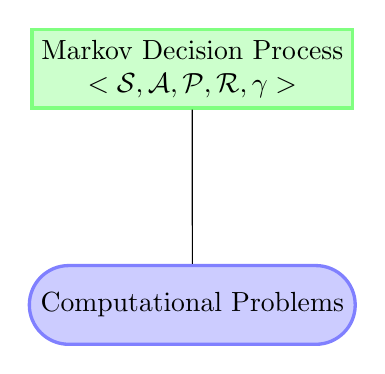
\begin{tikzpicture}
  [sibling distance = 10mm,
    level distance = 30mm,
    L1Node/.style={rounded rectangle, draw=blue!50, fill=blue!20, very thick, minimum size=10mm},
    L2Node/.style={rectangle, draw=green!50, fill=green!20, very thick, minimum size=10mm}]
    \node [L2Node, align=center]{Markov Decision Process\\$<\mathcal{S},\mathcal{A},\mathcal{P},\mathcal{R},\gamma>$}
    child { node[L1Node] {Computational Problems}
    };
\end{tikzpicture}

\end{document}
